\section{Wyniki części praktycznej}
W poprzednim rozdziale, omówione zostały operacje, techniki oraz technologie zastosowane przy implementacji poszczególnych modułów algorytmu. Po połączeniu ich w całość, otrzymujemy algorytm pozwalający na wykrycie samochodu w obrazie oraz rozpoznanie jego koloru. Aby móc ocenić poprawność oraz szybkość jego działania możemy posłużyć się wachlarzem przeznaczonych do tego celu metryk. 

Pierwsza kategoria testów to testy \textbf{funkcjonalne} - mówią one o tym, w jakim stopniu algorytm spełnia powierzone mu zadanie. 

Następnie przybliżony zostanie aspekt \textbf{wydajnościowy} wynikowego programu - to jak szybko działa jako zintegrowana całość, ale również wydajność jego wyodrębnionych modułów. W ten sposób możemy wywnioskować, które operacje należałoby zoptymalizować, by przynieść największy zysk wydajnościowy.

\subsection{Testy funkcjonalne}
Zadaniem zaprojektowanego algorytmu jest rozpoznawanie koloru samochodów osobowych z obrazu. Aby móc porównać ze sobą jakość i działanie wielu różnych implementacji opartych o uczenie maszynowe w jednolity sposób, ustandaryzowano kilka podstawowych metryk jakościowych. 

\subsubsection{Standardowe metryki}
\begin{description}
\item \textbf{Macierz pomyłek} (z ang. confusion matrix) - to podstawa do wyznaczenia metryk jakościowych uczenia maszynowego. Jest to macierz, która dla dwóch klas (prawda lub fałsz) przedstawia wartości:
\begin{description}
\item \textbf{Prawdziwy Pozytyw} (\textbf{TP} z ang. True Positive) - to prawidłowo sklasyfikowany wynik pozytywny.
\item \textbf{Prawdziwy Negatyw} (\textbf{TN} z ang. True Negative) - to prawidłowo sklasyfikowany wynik negatywny.
\item \textbf{Fałszywy Pozytyw} (\textbf{FP} z ang. False Positive) - to nieprawidłowo sklasyfikowany wynik pozytywny.
\item \textbf{Fałszywy Negatyw} (\textbf{FN} z ang. False Negative) - to nieprawidłowo sklasyfikowany wynik negatywny.
\end{description}

Macierz pomyłek przybiera rozmiary NxN, gdzie N to liczba klas.

\begin{table}[]
\begin{center}
\begin{tabular}{lc|cc|}
\cline{3-4}
\multicolumn{2}{l|}{\multirow{2}{*}{}}                                                                       & \multicolumn{2}{c|}{Przewidziany wynik}                                                                                                          \\ \cline{3-4} 
\multicolumn{2}{l|}{}                                                                                        & \multicolumn{1}{c|}{Prawda}                                                       & Fałsz                                                        \\ \hline
\multicolumn{1}{|c|}{\multirow{2}{*}{\begin{tabular}[c]{@{}c@{}}Prawdziwy\\ \\ wynik\end{tabular}}} & Prawda & \multicolumn{1}{c|}{\begin{tabular}[c]{@{}c@{}}Prawdziwy\\ Pozytyw\end{tabular}} & \begin{tabular}[c]{@{}c@{}}Fałszywy\\ Pozytyw\end{tabular}   \\ \cline{2-4} 
\multicolumn{1}{|c|}{}                                                                              & Fałsz & \multicolumn{1}{c|}{\begin{tabular}[c]{@{}c@{}}Fałszywy\\ Negatyw\end{tabular}}   & \begin{tabular}[c]{@{}c@{}}Prawdziwy \\ Negatyw\end{tabular} \\ \hline
\end{tabular}
\caption{Macierz pomyłek o rozmiarze 2x2}
\label{tab:Confusion2x2}
\end{center}
\end{table}

\pagebreak

\item \textbf{Dokładność} (z ang. accuracy) - to najpowszechniejsza miara jakości klasyfikacji. Jest to stosunek obiektów sklasyfikowanych poprawnie do wszystkich elementów zbioru. 
\begin{center}
\resizebox{0.45\hsize}{!}{
dokładność $= \frac{TP + TN}{TP + FP + FN + TN}$
}
\end{center}

\item \textbf{Precyzja} (z ang. precision) - to stosunek prawidłowo przewidzianych elementów klasy do wszystkich elementów zbioru sklasyfikowanych jako element tej klasy.
\begin{center}
\resizebox{0.3\hsize}{!}{
precyzja $= \frac{TP}{TP + FP}$
}
\end{center}

\item \textbf{Czułość} (z ang. recall) - to stosunek prawidłowo przewidzianych elementów klasy do wszystkich faktycznie należących do niej elementów.
\begin{center}
\resizebox{0.3\hsize}{!}{
czułość $= \frac{TP}{TP + FN}$
}
\end{center}

\item \textbf{Miara F$_{1}$} (z ang. F1 score) - to średnia harmoniczna precyzji i czułości.
\begin{center}
\resizebox{0.4\hsize}{!}{
F$_{1}$ $= \frac{2 \cdot precyzja \cdot czulosc}{precyzja + czulosc}$
}
\end{center}

\item \textbf{Wsparcie} (z ang. support) - to liczba elementów klasy w zbiorze, na podstawie których wyliczone zostały metryki dla danej klasy.
\end{description}

\subsubsection{Wyniki i wnioski}
Dla przypomnienia, w skład użytego zbioru danych wchodzi 8 klas kolorów. Macierz pomyłek, która opisuje klasyfikacje zaimplementowanego modelu ma zatem rozmiar 8x8.

\begin{figure}[h!]
    \begin{center}
        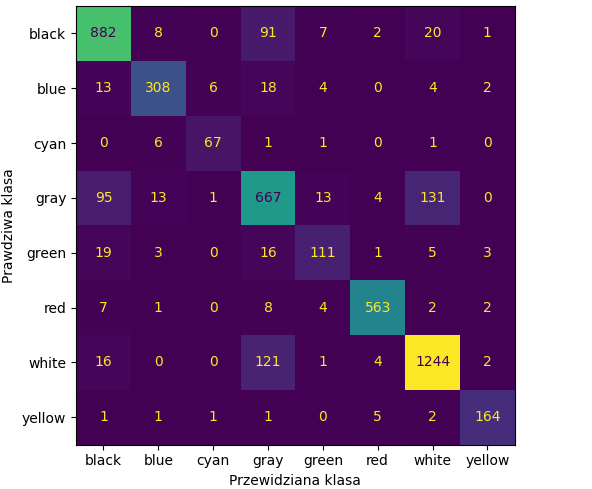
\includegraphics[scale=0.87]{img/confusion_matrix.png}        
    \end{center}
    \caption{Wynikowa macierz pomyłek}
    \label{fig:confusion_matrix}
\end{figure}

Wartości liczbowe zawarte w takiej macierzy pomyłek (Rysunek \ref{fig:confusion_matrix}) są jednak mało obrazowe. Jest tak, ponieważ każda z klas ma inne wsparcie. (Tabela \ref{tab:support})

\begin{table}[h!]
\begin{center}
\begin{tabular}{|l|l|l|l|l|l|l|l|}
\hline
Biały                      & Czarny                    & Szary                    & Czerwony                 & Niebieski                & Żółty                    & Zielony                  & Cyjanowy                \\ \hline
\multicolumn{1}{|c|}{1388} & \multicolumn{1}{c|}{1011} & \multicolumn{1}{c|}{924} & \multicolumn{1}{c|}{587} & \multicolumn{1}{c|}{355} & \multicolumn{1}{c|}{175} & \multicolumn{1}{c|}{158} & \multicolumn{1}{c|}{76} \\ \hline
\end{tabular}
\caption{Wsparcie klas}
\label{tab:support}
\end{center}
\end{table}

\begin{table}[h!]
\begin{center}
\begin{tabular}{|c|c|c|c|c|c|c|c|}
\hline
Biały & Czarny & Szary & Czerwony & Niebieski & Żółty & Zielony & Cyjanowy \\ \hline
4742  & 3418   & 3046  & 1941     & 1086      & 581   & 482     & 281      \\ \hline
\end{tabular}
\caption{Ilość elementów w każdej z klas}
\label{tab:classes_count}
\end{center}
\end{table}

Całkowite wsparcie, czyli ilość danych zbioru testowego, to \textbf{30\%} całkowitej ilości obrazów w zbiorze. Ta proporcja nie jest do końca zachowana dla każdej z klas i waha się w granicach \textbf{27,05\%} i \textbf{32,78\%}.

Możemy zatem w celu osiągnięcia bardziej obrazowej wizualizacji znormalizować macierz, tak, aby wyświetlane w niej wartości były niezależne od wsparcia poszczególnych klas.

\begin{figure}[h!]
    \begin{center}
        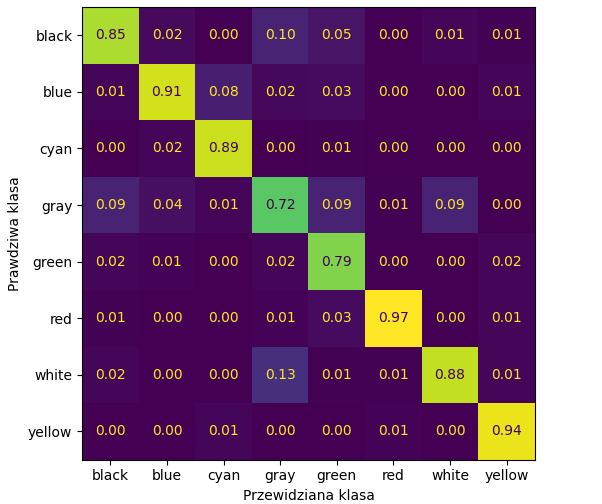
\includegraphics[scale=0.87]{img/confusion_matrix_new.png}        
    \end{center}
    \caption{Znormalizowana macierz pomyłek wobec ilości elementów przewidzianych jako należące do danej klasy}
    \label{fig:confusion_matrix_norm}
\end{figure}

\pagebreak

Z tak sformatowanej macierzy pomyłek (Rysunek \ref{fig:confusion_matrix_norm}) widzimy, że relatywnie najgorzej klasyfikowane były elementy klas kolorów: \textbf{zielony} oraz \textbf{szary}, a najwyższą jakościowo klasyfikacją wykazuje się klasa koloru \textbf{czerwonego}. Kolor szary najczęściej był mylony z kolorem (malejąco) białym, czarnym oraz zielonym. Natomiast kolor zielony najczęściej był mylony z kolorem zielonym oraz czarnym.
Podobny trend jest zauważalny na podstawie pozostałych metryk zawartych w poniższej tabeli (Tabela \ref{tab:metrics}).


\begin{table}[h!]
\begin{center}
\begin{tabular}{ccccc}
\cline{2-5}
\multicolumn{1}{c|}{}           & \multicolumn{1}{c|}{Precyzja} & \multicolumn{1}{c|}{Czułość} & \multicolumn{1}{c|}{Miara F1} & \multicolumn{1}{c|}{Wsparcie} \\ \hline
\multicolumn{1}{|c|}{Biały}     & \multicolumn{1}{c|}{0.88}     & \multicolumn{1}{c|}{0.90}    & \multicolumn{1}{c|}{0.89}     & \multicolumn{1}{c|}{1388}     \\ \hline
\multicolumn{1}{|c|}{Czarny}    & \multicolumn{1}{c|}{0.85}     & \multicolumn{1}{c|}{0.87}    & \multicolumn{1}{c|}{0.86}     & \multicolumn{1}{c|}{1011}     \\ \hline
\multicolumn{1}{|c|}{Szary}     & \multicolumn{1}{c|}{0.72}     & \multicolumn{1}{c|}{0.72}    & \multicolumn{1}{c|}{0.72}     & \multicolumn{1}{c|}{924}      \\ \hline
\multicolumn{1}{|c|}{Czerwony}  & \multicolumn{1}{c|}{0.97}     & \multicolumn{1}{c|}{0.96}    & \multicolumn{1}{c|}{0.97}     & \multicolumn{1}{c|}{587}      \\ \hline
\multicolumn{1}{|c|}{Niebieski} & \multicolumn{1}{c|}{0.91}     & \multicolumn{1}{c|}{0.87}    & \multicolumn{1}{c|}{0.89}     & \multicolumn{1}{c|}{355}      \\ \hline
\multicolumn{1}{|c|}{Żółty}     & \multicolumn{1}{c|}{0.94}     & \multicolumn{1}{c|}{0.94}    & \multicolumn{1}{c|}{0.94}     & \multicolumn{1}{c|}{175}      \\ \hline
\multicolumn{1}{|c|}{Zielony}   & \multicolumn{1}{c|}{0.79}     & \multicolumn{1}{c|}{0.70}    & \multicolumn{1}{c|}{0.74}     & \multicolumn{1}{c|}{158}      \\ \hline
\multicolumn{1}{|c|}{Cyjanowy}  & \multicolumn{1}{c|}{0.89}     & \multicolumn{1}{c|}{0.88}    & \multicolumn{1}{c|}{0.89}     & \multicolumn{1}{c|}{76}       \\ \hline
\multicolumn{1}{|c|}{Średnia}   & \multicolumn{1}{c|}{0.87}     & \multicolumn{1}{c|}{0.85}    & \multicolumn{1}{c|}{0.86}     & \multicolumn{1}{c|}{4674}     \\ \hline
\multicolumn{1}{l}{}            & \multicolumn{1}{l}{}          & \multicolumn{1}{l}{}         & \multicolumn{1}{l}{}          & \multicolumn{1}{l}{}          \\ \hline
\multicolumn{2}{|l|}{\textbf{Dokładność}}                       & \multicolumn{3}{c|}{\textbf{86.24\%}}                                                        \\ \hline
\end{tabular}
\caption{Metryki jednowymiarowe}
\label{tab:metrics}
\end{center}
\end{table}

\pagebreak

Niskie rezultaty jakościowe dla najgorzej klasyfikowanych kolorów, są spowodowane w dużej mierze degeneracją i błędami w zbiorze danych. Jako dowód można przytoczyć zrzut ekranu zawartości folderu, w którym znajdują się zdjęcia samochodów z etykietą koloru \textbf{"\null{}green"} (zielone auta):

\begin{figure}[h!]
    \begin{center}
        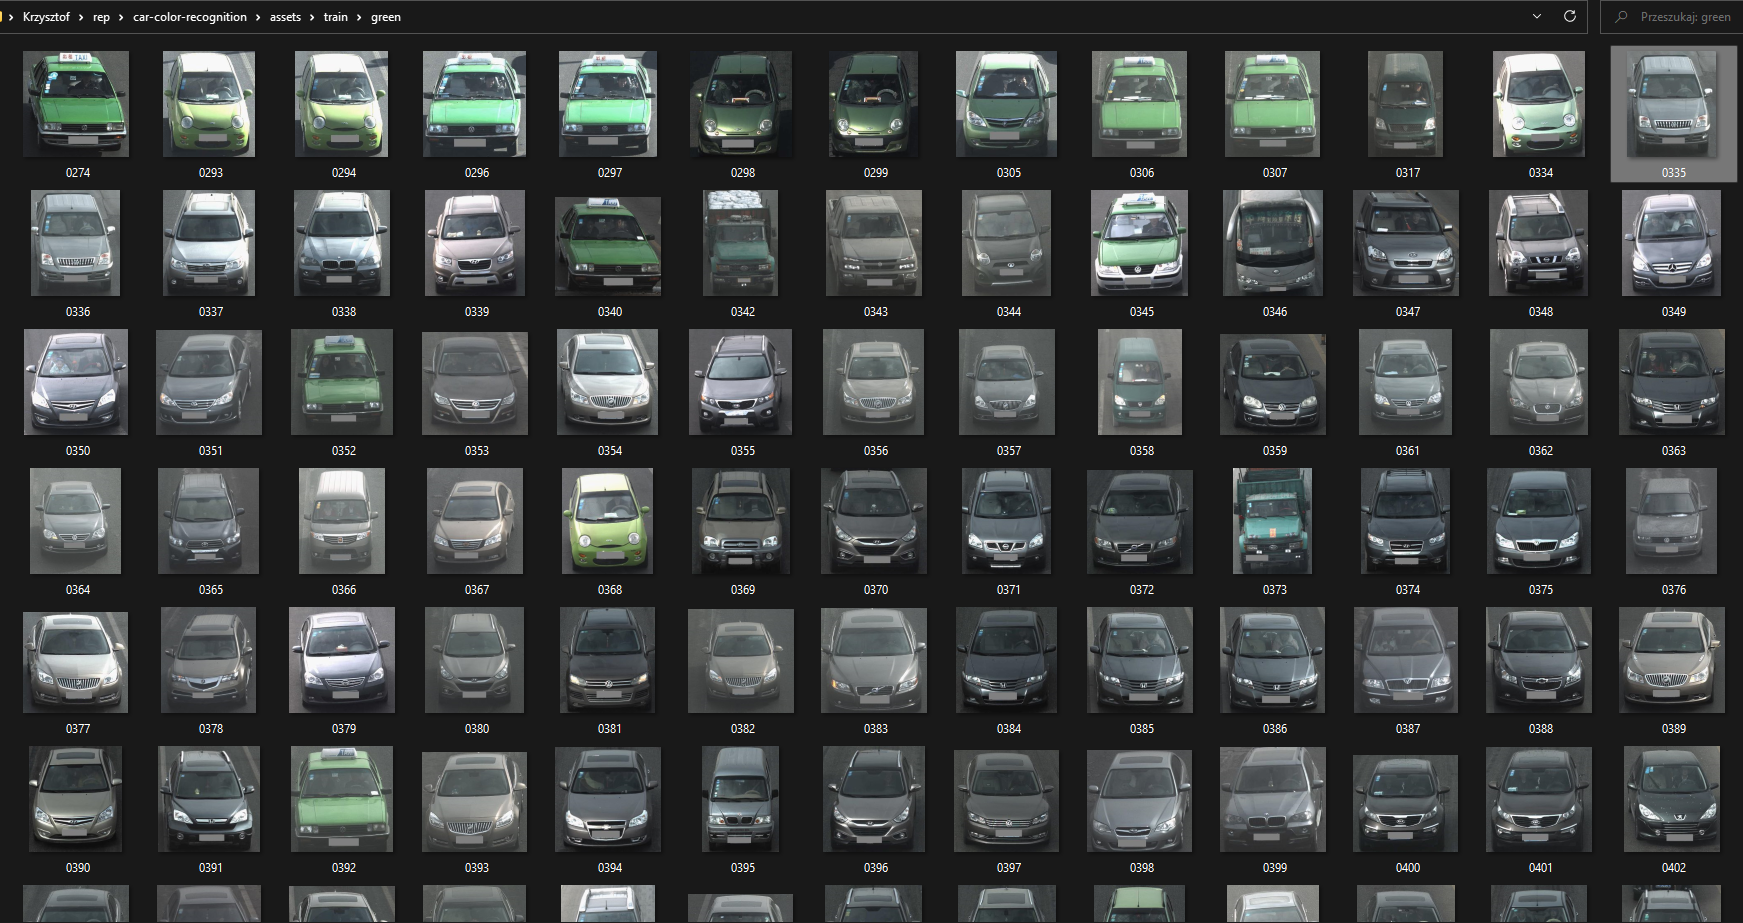
\includegraphics[scale=0.31]{img/green_cars_xd.png}        
    \end{center}
    \caption{Katalog zawierający zdjęcia aut opisane jako zielone}
    \label{fig:green_cars_xd}
\end{figure}

Ogromna ilość z widocznych w katalogu zdjęć, zawiera auta o kolorze szarym i czarnym, a \textbf{nie zielonym}. Nie powinno być więc zaskoczeniem, iż auta zielone są mylone często z autami czarnymi oraz szarymi, skoro duża część etykiet jest kompletnie \underline{źle przypisana}. 

\begin{figure}[h!]
    \begin{center}
        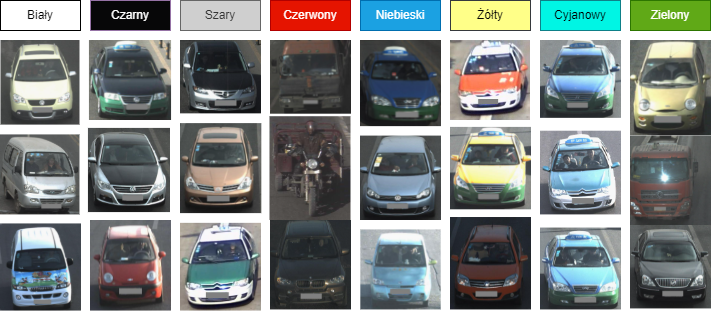
\includegraphics[scale=0.57]{img/cars_bad_colors.png}        
    \end{center}
    \caption{Po 3 przykładowe, źle przypisane elementy dla każdej z klas}
    \label{fig:bad_cars_xd}
\end{figure}

Podobnie jak kolor zielony, inne klasy mają dużo źle przypisanych elementów, co widać na powyższym rysunku (Rysunek \ref{fig:bad_cars_xd}). Do wizualizacji zostało wybrane tylko kilka najbardziej rażących przypadków z każdej z klas (bez powtórek tego samego auta - mimo, że każde występuje kilku lub kilkunastokrotnie w zbiorze oryginalnym).

Aby zniwelować ten problem, zbiór danych został manualnie wyczyszczony, to znaczy pozbawiony zdjęć, których etykiety były sprzeczne z rzeczywistością obrazu. Takich przypadków było niestety dużo, co poskutkowało znacznym zmniejszeniem się wynikowej ilości elementów zbioru. Zmniejszyła się ona z ponad \textbf{15 tys.} obrazów, do tylko \textbf{6415} zdjęć.

\begin{table}[h!]
\begin{center}
\begin{tabular}{|c|c|c|c|c|c|c|c|}
\hline
Biały & Czarny & Szary & Czerwony & Niebieski & Żółty & Cyjanowy & Zielony \\ \hline
739   & 726    & 469   & 145      & 66        & 38    & 32       & 31      \\ \hline
\end{tabular}
\caption{Wsparcie klas po czyszczeniu zbioru danych}
\label{tab:support_reword}
\end{center}
\end{table}

Stosunek podziału zbioru na dane trenujące i testowe został zmieniony z \textbf{70:30} do \textbf{65:35}, a mimo tego, wsparcie niektórych klas i tak stało się na tyle małe, że może ono budzić niepewność i podejrzliwość co do uzyskanych wyników jakościowych.

\begin{table}[h!]
\begin{center}
\begin{tabular}{|c|c|c|c|c|c|c|c|}
\hline
Biały & Czarny & Szary & Czerwony & Niebieski & Żółty & Cyjanowy & Zielony \\ \hline
2153  & 1972   & 1318  & 449      & 217       & 121   & 107      & 78      \\ \hline
\end{tabular}
\caption{Ilości elementów poszczególnych klas zbioru po jego czyszczeniu}
\label{tab:dataset_count_reword}
\end{center}
\end{table}

Po usunięciu ze zbioru obrazów o sprzecznych etykietach lub nie-akceptowalnych jakościowo zdjęć (takich, w których koloru auta nie rozpoznałby nawet człowiek), otrzymujemy następujące macierze pomyłek oraz metryki jednowymiarowe:

\begin{table}[h!]
\begin{center}
\begin{tabular}{crrrr}
\cline{2-5}
\multicolumn{1}{c|}{}           & \multicolumn{1}{c|}{Precyzja} & \multicolumn{1}{c|}{Czułość} & \multicolumn{1}{c|}{Miara F1} & \multicolumn{1}{c|}{Wsparcie} \\ \hline
\multicolumn{1}{|c|}{Biały}     & \multicolumn{1}{r|}{0.97}     & \multicolumn{1}{r|}{0.82}    & \multicolumn{1}{r|}{0.89}     & \multicolumn{1}{r|}{726}      \\ \hline
\multicolumn{1}{|c|}{Czarny}    & \multicolumn{1}{r|}{0.96}     & \multicolumn{1}{r|}{0.96}    & \multicolumn{1}{r|}{0.96}     & \multicolumn{1}{r|}{66}       \\ \hline
\multicolumn{1}{|c|}{Szary}     & \multicolumn{1}{r|}{0.91}     & \multicolumn{1}{r|}{0.93}    & \multicolumn{1}{r|}{0.92}     & \multicolumn{1}{r|}{32}       \\ \hline
\multicolumn{1}{|c|}{Czerwony}  & \multicolumn{1}{r|}{0.99}     & \multicolumn{1}{r|}{0.99}    & \multicolumn{1}{r|}{0.99}     & \multicolumn{1}{r|}{469}      \\ \hline
\multicolumn{1}{|c|}{Niebieski} & \multicolumn{1}{r|}{0.89}     & \multicolumn{1}{r|}{0.94}    & \multicolumn{1}{r|}{0.91}     & \multicolumn{1}{r|}{31}       \\ \hline
\multicolumn{1}{|c|}{Żółty}     & \multicolumn{1}{r|}{0.97}     & \multicolumn{1}{r|}{0.82}    & \multicolumn{1}{r|}{0.89}     & \multicolumn{1}{r|}{145}      \\ \hline
\multicolumn{1}{|c|}{Zielony}   & \multicolumn{1}{r|}{0.93}     & \multicolumn{1}{r|}{0.81}    & \multicolumn{1}{r|}{0.86}     & \multicolumn{1}{r|}{739}      \\ \hline
\multicolumn{1}{|c|}{Cyjanowy}  & \multicolumn{1}{r|}{0.91}     & \multicolumn{1}{r|}{0.94}    & \multicolumn{1}{r|}{0.92}     & \multicolumn{1}{r|}{38}       \\ \hline
\multicolumn{1}{|c|}{Średnia}   & \multicolumn{1}{r|}{0.94}     & \multicolumn{1}{r|}{0.92}    & \multicolumn{1}{r|}{0.93}     & \multicolumn{1}{r|}{2246}     \\ \hline
\multicolumn{1}{l}{}            & \multicolumn{1}{l}{}          & \multicolumn{1}{l}{}         & \multicolumn{1}{l}{}          & \multicolumn{1}{l}{}          \\ \hline
\multicolumn{2}{|l|}{\textbf{Dokładność}}                       & \multicolumn{3}{c|}{\textbf{95.32\%}}                                                        \\ \hline
\end{tabular}
\caption{Metryki jednowymiarowe po czyszczeniu zbioru danych}
\label{tab:metrics_reword}
\end{center}
\end{table}

\pagebreak

\begin{figure}[h!]
    \begin{center}
        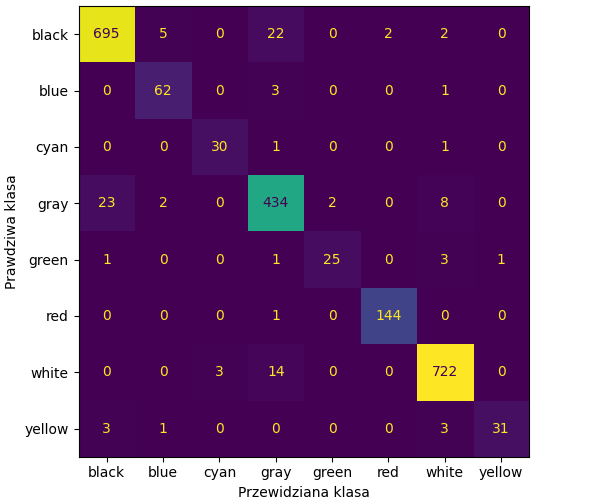
\includegraphics[scale=0.78]{img/confusion_matrix_rework.png}        
    \end{center}
    \caption{Macierz pomyłek po czyszczeniu zbioru}
    \label{fig:confusion_rework}
\end{figure}

\begin{figure}[h!]
    \begin{center}
        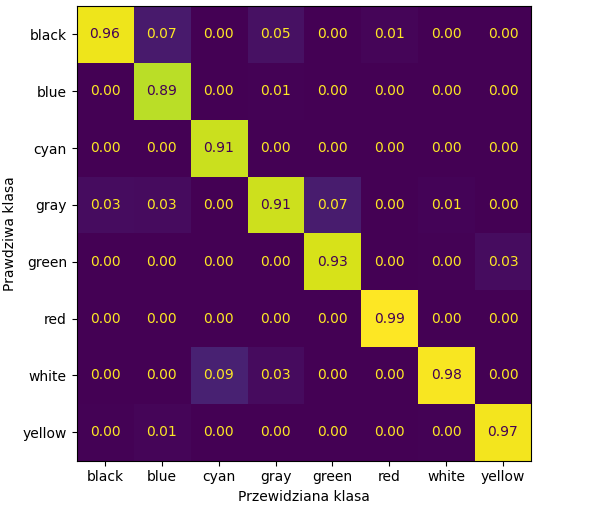
\includegraphics[scale=0.78]{img/confusion_matrix_new_rework.png}
    \end{center}
    \caption{Znormalizowana macierz pomyłek po czyszczeniu zbioru}
    \label{fig:confusion_new_rework}
\end{figure}

\pagebreak

Są to bardzo obiecujące wyniki, przewyższające te, osiągnięte w realizacji opisanych wcześniej prac naukowych, które korzystają z tego zbioru danych. Zbiór danych przy trenowaniu modelu jest dzielony na dwa osobne, niezależne podzbiory - \textbf{trenujący} i \textbf{testujący}. Przez ten fakt możemy z wysokich wyników jakościowych wysnuć wniosek, że model poprawnie uogólnia nowo napotkane, nieznane mu przypadki aut.

Trzeba jednak mieć na uwadze, że wszystkie podane metryki są miarą tego jak dobrze model generalizuje auta ze zdjęć zbioru testowego. Zatem dobrze wypadający na takich testach model cechujący się dokładnością nieco ponad \textbf{95\%}, może wykazywać się ubogą jakością generalizacji na danych spoza zbioru testowego, na przykład danych rzeczywistych.

\subsection{Testy wydajnościowe}
Oprócz informacji o tym \textbf{co?}, \textbf{jak?} i \textbf{w jakim stopniu?} robi algorytm, chcielibyśmy uzyskać również wgląd w to w jakim czasie potrafi osiągnąć daną funkcjonalność. Kroki algorytmu wpływają w jego holistyczny czas wykonania w różnym stopniu. Przetestowane pod kątem wydajnościowym zostaną zatem najbardziej znaczące moduły, takie jak trenowanie modelu, detekcja pojazdów oraz działanie programu jako całość.

Wszystkie parametry czasowe były pozyskiwane na komputerze stacjonarnym z użyciem jedynie \textbf{CPU}. Jest to spowodowane poważnymi problemami z uruchomieniem modułu OpenCV w wersji używającej wspomagania dedykowanego układu GPU z rdzeniami CUDA w celu dalszego zrównoleglenia obliczeń. 

\subsubsection{Czas trenowania modelu}
Istnieją dwie wersje modelu perceptronu wielowarstwowego, którego używa algorytm. Jest to model przed i po czyszczeniu zbioru danych. Przed czyszczeniem zbioru, składał się on z \textbf{15579} obrazów. Wtedy czas uczenia modelu wahał się w granicach \textbf{260-310 sekund}, czyli około czterech minut.

Po czyszczeniu zbioru danych, jego liczebność zmalała do 6415 obrazów. Przy takiej ilości zdjęć, czas potrzebny na wytrenowanie perceptronu wielowarstwowego zawierał się w granicach \textbf{70-120 sekund}.

Oba czasy, przed i po zmianie zbioru danych, są o kilka rzędów niższe od czasu potrzebnego na trenowanie modelu w rozwiązaniach opartych o CNN, które przy około 8 tysiącach obrazów trwało niemal 4 dni (na potężnym komputerze dysponującym drogimi zestawami GPU!), a tak czy inaczej uzyskało wynik \textbf{94\%} dokładności generalizacji, czyli \textbf{niższy o 1\%} od uzyskanego modelu.

\subsubsection{Szybkość detekcji}
Program pozwala nam na dokonanie detekcji samochodów osobowych na trzech typach danych wejściowych: z zapisanego na dysku obrazu, z zapisanego na dysku obrazu wideo lub obrazu na żywo z systemowego wejścia wideo.

Dla obrazów stałych, miarą szybkości detekcji może być po prostu sumaryczny czas potrzebny na odnalezienie, obróbkę (wskazanie) oraz wyświetlenie obrazu wynikowego. Czas ten zawiera się w granicach \textbf{360-450 milisekund}, przy 20 próbach. Średnia czasu z wszystkich prób to: \textbf{387.2 milisekundy}.

Dla obrazów wideo oraz obrazu na żywo, obraną miarą szybkości detekcji są klatki na sekundę (FPS, z and. Frames per Second). Jednak miara FPS rzadko jest stała przez czas całość trwania wideo. Dlatego podana zostanie \textbf{wartość średnia} FPS, \textbf{mediana}, \textbf{wartość maksymalna} oraz \textbf{25.} oraz \textbf{75. centyl}.

\begin{description}
\item \textbf{Wideo nr1} - przypadek testowy numer 1. To 10 sekundowy film przedstawiający obraz z ruchomej kamery ulicznej pozycjonowanej nad czteropasmową drogą szybkiego ruchu z widokiem frontalnym na nadjeżdżające samochody osobowe. Na filmie przez pole widzenia kamery przejeżdża wiele aut i widocznych jest wiele innych obiektów przyulicznych. Rozdzielczość obrazu to 1280x720 pikseli, a oryginalna ilość klatek na sekundę to 29.97 FPS.

\item \textbf{Wideo nr2} - przypadek testowy numer 2. To krótkie, 5 sekundowe wideo, w którym widać od przodu wchodzące w zakręt i z niego wychodzące pojedyncze niebieskie auto. Dookoła widać dużo przedmiotów przyulicznych i roślinności. Rozdzielczość filmu to 960x540, w oryginale 30 FPS. 

\end{description}

\begin{table}[h!]
\begin{center}
\begin{tabular}{|l|l|l|}
\hline
\multicolumn{1}{|c|}{Miary FPS} & Wideo nr1 & Wideo nr2 \\ \hline
Średnia                         & \textbf{5.245}     & \textbf{5.040}     \\ \hline
Max                             & 5.579     & 5.465     \\ \hline
75.                             & 5.404     & 5.212     \\ \hline
Mediana                         & 5.265     & 5.151     \\ \hline
25.                             & 5.163     & 4.927     \\ \hline
\end{tabular}
\caption{Miary FPS detekcji z obrazu wideo dla dwóch przypadków testowych}
\label{tab:fps_detection}
\end{center}
\end{table}

\begin{figure}[h!]
    \begin{center}
        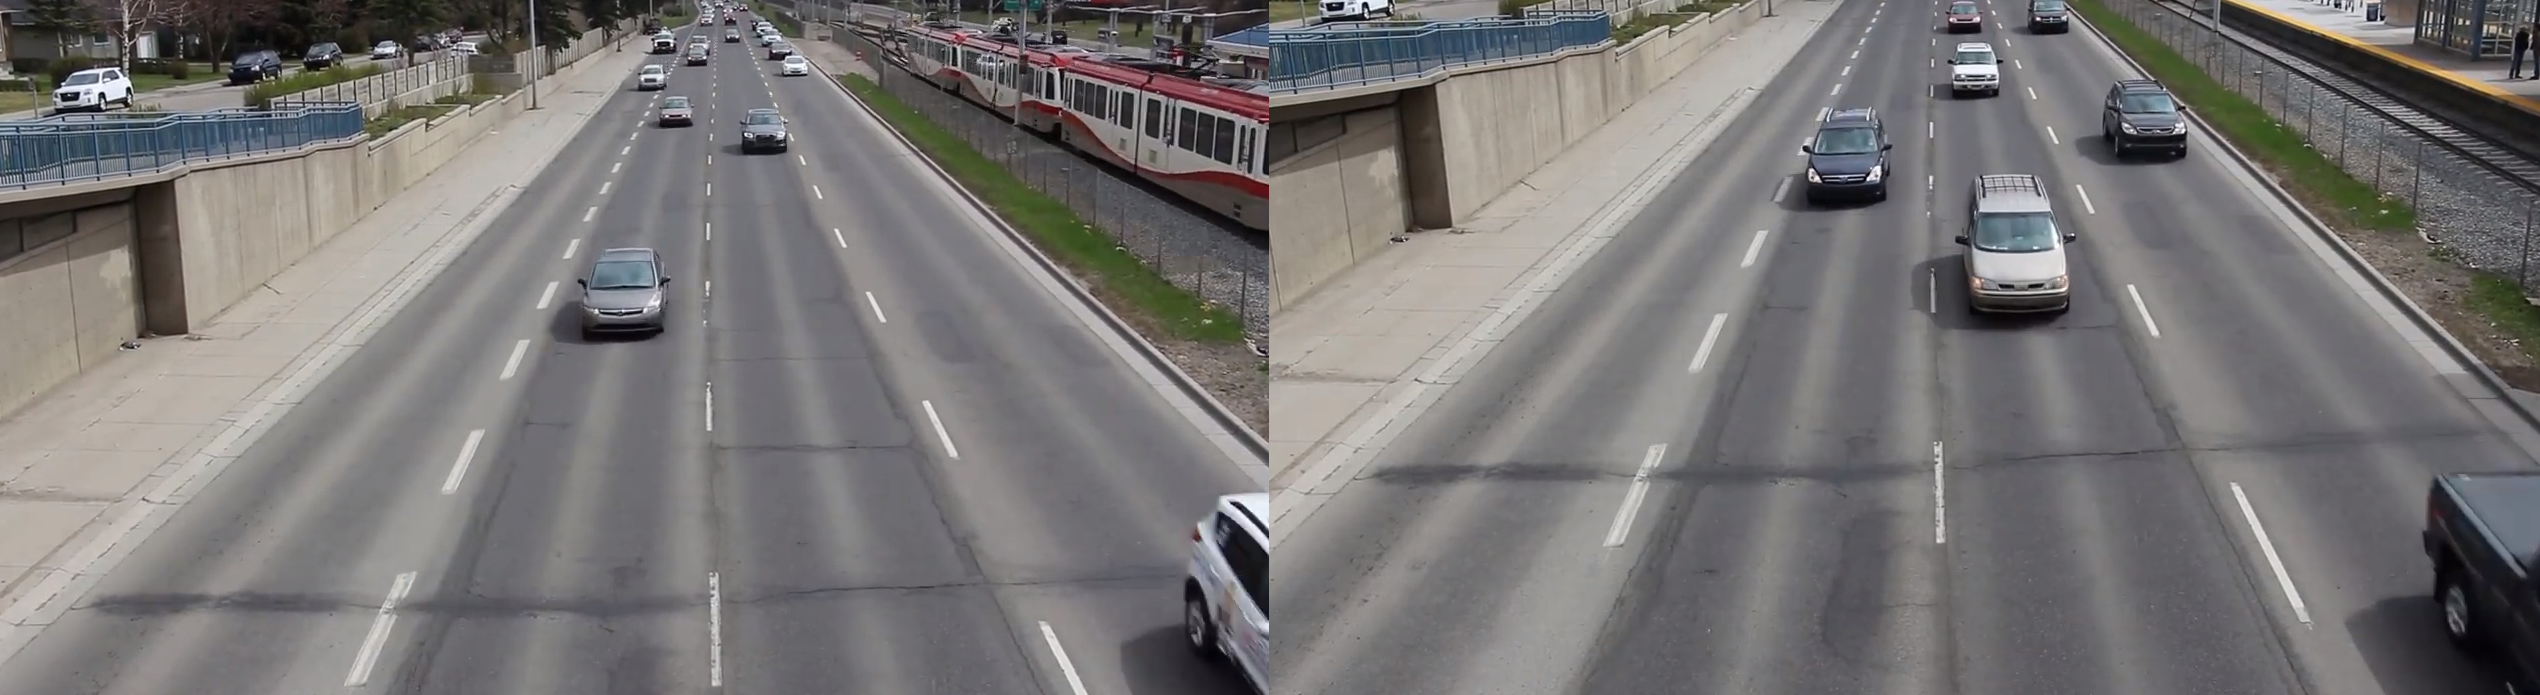
\includegraphics[scale=0.21]{img/cam1.png}
    \end{center}
    \caption{Dwa przykładowe ujęcia z przypadku testowego nr1}
    \label{fig:cam1}
\end{figure}

\begin{figure}[h!]
    \begin{center}
        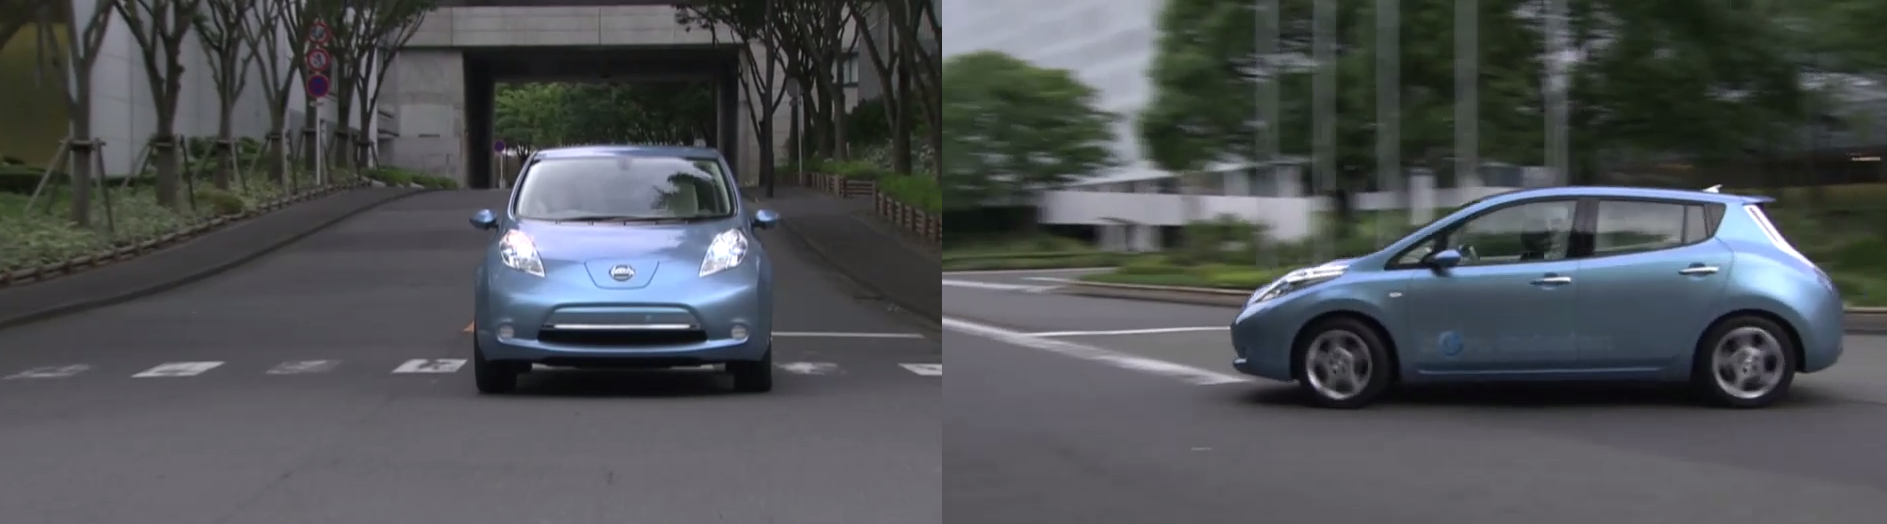
\includegraphics[scale=0.28]{img/cam2.png}
    \end{center}
    \caption{Dwa przykładowe ujęcia z przypadku testowego nr2}
    \label{fig:cam2}
\end{figure}

% Opis wynikow

\pagebreak

\subsubsection{Parametry czasowe rozpoznawania koloru samochodów}

Parametry czasowe działania całości algorytmu, czyli detekcji i rozpoznawania koloru samochodów osobowych już wytrenowanym modelem, pozyskiwane są analogiczne do parametrów czasowych samej detekcji.

Dla obrazów stałych, jest to czas potrzebny na użycie algorytmu na zdjęciach. Wartość tego czasu zawiera się w granicach \textbf{455-584 milisekund}, przy 20 próbach. Średnia czasu z wszystkich prób to: \textbf{483.1 milisekundy}.\\

Natomiast dla obrazów wideo jak i obrazu "\null{}na żywo", pozyskane parametry czasowe prezentują się następująco:

\begin{table}[h!]
\begin{center}
\begin{tabular}{|l|l|l|}
\hline
\multicolumn{1}{|c|}{Miary FPS} & Wideo nr1 & Wideo nr2 \\ \hline
Średnia                         & \textbf{4.571}     & \textbf{4.826}     \\ \hline
Max                             & 5.256     & 5.190     \\ \hline
75.                             & 4.877     & 4.993     \\ \hline
Mediana                         & 4.756     & 4.849     \\ \hline
25.                             & 4.540     & 4.774     \\ \hline
\end{tabular}%
\caption{Miary FPS działania pełnego algorytmu na obrazie wideo dla dwóch przypadków testowych}
\label{tab:fps_recog}
\end{center}
\end{table}

Widać zatem, iż to detekcja jest najbardziej obarczającą algorytm czasowo operacją. Zmniejszenie czasu potrzebnego na detekcję pod kątem oprogramowania, wiązałoby się z użyciem innych parametrów modelu detekcji, stworzeniem zupełnie innego modelu lub skorzystanie z zupełnie innego rozwiązania niż uczenie maszynowe. Inny sposób to podejście sprzętowe. Użycie układu GPU obsługującego technologie CUDA, w celu zrównoleglenia obliczeń znacznie wpłynęłoby na całościową szybkość działania algorytmu. 

Niestety, dostępne stacje robocze oraz zasoby komputerowe nie pozwalają mi na użycie układu GPU z moim programem. To znacznie zmniejsza atrakcyjność algorytmu w kontekście jego działania na obrazie wideo.